% =====================================================================
% ViAmpleHate — Bản dịch tiếng Việt của bài báo ACL (latex_vi)
% Dịch từ paper/main/latex/acl_latex.tex. Các thuật ngữ kỹ thuật IT/ML
% (encoder, attention, relation-bank attention, target-cue/attack-cue bank,
% gate, classifier, baseline, contrastive, cross-entropy, token, embedding,
% batch, query/key/value, residual...) được GIỮ NGUYÊN tiếng Anh, chỉ dịch
% phần văn xuôi và các từ phổ thông. Số liệu, công thức, nhãn NON-HATE/HATE,
% tên mô hình và trích dẫn giữ nguyên như bản gốc.
% Đã áp dụng cùng các chỉnh sửa với bản tiếng Anh:
%   - Bỏ mục Limitations và Ethics Statement.
%   - Gộp Mục 6 (Kết quả và Phân tích) và Mục 7 (Phân tích lỗi)
%     thành "Kết quả và Phân tích lỗi".
% TRÌNH BIÊN DỊCH: biên dịch được bằng CẢ pdfLaTeX lẫn XeLaTeX/LuaLaTeX.
%   - pdfLaTeX: dùng [T5]{fontenc} + [utf8]{inputenc} + lmodern (qua iftex).
%   - XeLaTeX/LuaLaTeX: dùng fontspec với phông Latin Modern Roman.
% Cần: acl.sty, acl_natbib.bst (từ template ACL) + custom.bib (trong thư mục này).
% =====================================================================
\documentclass[11pt]{article}

\usepackage[final]{acl}  % hiện tên tác giả (dùng "review" cho bản ẩn danh)

\usepackage{latexsym}
% --- Hỗ trợ tiếng Việt cho CẢ pdfLaTeX lẫn XeLaTeX/LuaLaTeX ---
\usepackage{iftex}
\ifPDFTeX
  \usepackage[utf8]{inputenc}
  \usepackage[T5]{fontenc}   % T5 = bảng mã tiếng Việt cho pdfLaTeX
  \usepackage{lmodern}       % Latin Modern: đủ glyph tiếng Việt trong T5
\else
  \usepackage{fontspec}            % XeLaTeX/LuaLaTeX
  \setmainfont{Latin Modern Roman} % đủ dấu tiếng Việt
\fi
\usepackage{microtype}
\usepackage{graphicx}
\usepackage{amsmath}
\usepackage{amssymb}
\usepackage{booktabs}
\usepackage{array}
\usepackage{float}
\usepackage{tikz}
\usetikzlibrary{arrows.meta,positioning,fit,backgrounds,calc}

\title{ViAmpleHate: Một hướng tiếp cận dựa trên AmpleHate và PhoBERT\\ cho bài toán phát hiện phát ngôn thù ghét tiếng Việt}

\author{
  \textbf{Tran Nguyen Duc Trung} \quad
  \textbf{Nguyen Ha Minh Tuan} \quad
  \textbf{Nguyen Gia Cat Long} \\
  \textbf{Tran Phan Thanh Tung} \quad
  \textbf{Mo Van Tung} \\[4pt]
  Trường Đại học Công nghệ Thông tin, ĐHQG-HCM, Thành phố Hồ Chí Minh, Việt Nam \\
  \texttt{\{23521687, 23521718, 23520881, 23521747, 23521741\}@gm.uit.edu.vn}
}

\setlength\titlebox{6cm}

\begin{document}
\maketitle

\begin{abstract}
Phát hiện phát ngôn thù ghét trên mạng xã hội tiếng Việt là một bài toán khó, vì ý đồ thù ghét không phải lúc nào cũng xuất hiện qua thực thể có tên mà thường ẩn trong cách gọi nhóm phi chính thức, tiếng lóng, mỉa mai và các ám chỉ gián tiếp. Các mô hình \emph{target-aware} như AmpleHate cho thấy việc đưa quan hệ giữa phát ngôn và đối tượng bị nhắm tới vào cơ chế attention có thể hỗ trợ phát hiện cả những trường hợp thù ghét hàm ẩn. Tuy nhiên, pipeline gốc của AmpleHate phụ thuộc vào NER tiếng Anh và các phạm trù target được thiết kế cho tiếng Anh, nên khi chuyển sang tiếng Việt, hiệu quả suy giảm đáng kể: trên tập huấn luyện của nhóm, NER tiếng Anh chỉ tìm được target khả dụng trong khoảng 0,09\% bình luận, khiến mô hình gần như thoái hóa thành một classifier ở mức câu.
Nhóm đề xuất \textbf{ViAmpleHate}, một phiên bản thích ứng của AmpleHate cho tiếng Việt trên nền PhoBERT, với bốn thay đổi chính: (i) thay NER tiếng Anh bằng NER tiếng Việt kết hợp một \emph{target-cue bank} được tuyển chọn, qua đó nâng độ phủ target lên khoảng 19--45\% tùy bộ dữ liệu; (ii) bổ sung một \emph{attack-cue bank} riêng và mô hình hóa ba kênh quan hệ---target tường minh, context hàm ẩn và attack---bằng \emph{relation-bank attention}; (iii) thay phép injection cố định bằng \emph{instance-adaptive gate}; và (iv) huấn luyện bằng weighted cross-entropy kết hợp contrastive loss.
Trên ViHSD và VOZ-HSD, trong thiết lập nhị phân NON-HATE/HATE, ViAmpleHate cải thiện cả macro-F1 lẫn HATE-F1 so với baseline AmpleHate cũng như các baseline TF-IDF, BiLSTM và PhoBERT-CNN; mức tăng rõ nhất nằm ở lớp thiểu số (HATE-F1 tăng $0{,}0508$ trên VOZ-HSD). Riêng trên ViHSD, mức cải thiện còn nhỏ, nên nhóm xem đây là kết quả sơ bộ và cần kiểm chứng thêm bằng đánh giá đa seed có kiểm soát. Phân tích bổ sung cho thấy độ phủ target-cue có liên hệ với mức cải thiện; kết quả này ủng hộ nhận định rằng mô hình target-aware cần được thích ứng với tiếng Việt thay vì chuyển nguyên xi từ tiếng Anh, dù chưa đủ để khẳng định quan hệ nhân quả.
\end{abstract}

\section{Giới thiệu}

Sự phát triển nhanh của mạng xã hội tiếng Việt đi kèm với sự lan rộng của nội dung thù ghét và lăng mạ. Những nội dung này gây hại cho cá nhân, cộng đồng bị nhắm tới, đồng thời tạo rủi ro pháp lý và danh tiếng cho các nền tảng. Khi lượng nội dung vượt xa khả năng kiểm duyệt thủ công, phát hiện phát ngôn thù ghét tự động trở thành nhu cầu cấp thiết. Tuy nhiên, phần lớn tiến bộ hiện nay vẫn tập trung ở tiếng Anh và các ngôn ngữ giàu tài nguyên; khi áp dụng sang tiếng Việt, hiệu quả thường giảm đáng kể.

Phát hiện phát ngôn thù ghét tiếng Việt khó vì ba lý do đan xen. Thứ nhất, ngôn ngữ trên mạng xã hội rất nhiễu: người dùng viết tắt, dùng \emph{teencode}, kéo dài ký tự, chèn emoji mang sắc thái ngữ dụng và viết sai chính tả, đôi khi còn cố tình che lời tục để né bộ lọc. Thứ hai, và cũng là điểm quan trọng nhất, \emph{target} của một lời công kích hiếm khi là một thực thể có tên. Nếu trong tiếng Anh, phát ngôn thù ghét thường gọi đích danh một cá nhân, tổ chức hoặc quốc tịch, thì trong tiếng Việt sự thù địch thường hướng tới cả một nhóm thông qua đại từ, danh từ thân tộc hay danh từ chỉ nhóm, nhãn vùng miền hoặc các lối xưng hô phi chính thức. Thứ ba, dữ liệu bị mất cân bằng mạnh: ở cả hai bộ dữ liệu, lớp HATE chỉ chiếm khoảng một phần mười, nên mô hình vẫn có thể đạt accuracy cao dù gần như không phát hiện được trường hợp thù ghét nào.

Một hướng tiếp cận hứa hẹn là mô hình hóa phát ngôn thù ghét theo kiểu \emph{target-aware}. AmpleHate \citep{amplehate} cho thấy attention tường minh vào quan hệ giữa câu và target tiềm năng giúp phát hiện tốt hơn thù ghét \emph{hàm ẩn}, tức những trường hợp không có slur lộ liễu. Cụ thể, mô hình trích các target ứng viên bằng NER, tính một attention vector target-aware rồi inject vector này vào biểu diễn câu trước khi phân loại. Hướng này phù hợp với tiếng Việt, nơi target thường giữ vai trò trung tâm, nhưng pipeline gốc lại dựa trên NER và phạm trù target của tiếng Anh. Khi chạy trên tiếng Việt với NER tiếng Anh, hệ thống chỉ tìm được target khả dụng ở 21/24{.}048 bình luận huấn luyện (khoảng 0,09\%); vì vậy, phần lớn đầu vào phải quay về biểu diễn toàn cục \texttt{[CLS]}, khiến mô hình gần như hoạt động như một PhoBERT classifier thông thường và đánh mất tín hiệu target-aware vốn là động lực chính.

Nhóm đề xuất \textbf{ViAmpleHate}, một phiên bản thích ứng của AmpleHate cho tiếng Việt, trong đó từng khâu của pipeline được điều chỉnh để phù hợp hơn với cách người Việt biểu đạt sự thù ghét trên mạng xã hội. Các đóng góp chính gồm:
\begin{enumerate}
  \item \textbf{Trích xuất target tiếng Việt.} Nhóm thay NER tiếng Anh bằng một mô hình NER tiếng Việt kết hợp với \emph{target-cue bank} được tuyển chọn (gồm đại từ, danh từ chỉ nhóm và các lối xưng hô phi chính thức), qua đó nâng tỷ lệ bình luận phát hiện được target từ khoảng 0,09\% lên 18,8--20,0\%.
  \item \textbf{Tách riêng kênh target và kênh attack.} Nhóm bổ sung một \emph{attack-cue bank} cho các vị từ thù địch, đồng thời xử lý cue target và cue attack như hai tín hiệu độc lập trong một \textbf{relation-bank attention} ba kênh.
  \item \textbf{Fusion thích ứng (kèm ghi chú triển khai).} Nhóm thay phép injection cố định theo hệ số vô hướng của AmpleHate bằng \textbf{instance-adaptive gate}; ngoài ra, bài báo ghi nhận một chỉnh sửa ở mức triển khai cho phép tính attention theo batch trong bản port (chỉ xem là ghi chú triển khai, không phải đóng góp chính).
  \item \textbf{Hàm mục tiêu huấn luyện.} Nhóm kết hợp weighted cross-entropy với contrastive loss để làm rõ hơn ranh giới giữa HATE và NON-HATE trong điều kiện mất cân bằng.
  \item \textbf{Nghiên cứu thực nghiệm.} Nhóm đánh giá trên ViHSD và VOZ-HSD với năm baseline, đồng thời phân tích nguồn gốc của các mức cải thiện, bao gồm độ phủ target và khảo sát định tính những lỗi còn lại.
\end{enumerate}
target-aware là một inductive bias hữu ích cho bài toán phát hiện phát ngôn thù ghét, nhưng chỉ phát huy đầy đủ khi được thích ứng với đặc trưng bề mặt của ngôn ngữ đích, thay vì chuyển nguyên xi từ tiếng Anh.

\section{Công trình liên quan}

\subsection{Phát hiện phát ngôn thù ghét và thù ghét hàm ẩn}
Các phương pháp phát hiện phát ngôn thù ghét tự động đã phát triển từ classifier dựa trên từ điển và đặc trưng thủ công, qua các mô hình chuỗi sâu, đến các transformer tiền huấn luyện gần đây. Một trở ngại dai dẳng là thù ghét \emph{hàm ẩn}: thông điệp thể hiện sự thù địch mà không dùng slur tường minh, thay vào đó dựa vào mỉa mai, định kiến, tham chiếu được mã hóa hoặc kiến thức nội nhóm. Dạng này thường gặp hơn slur lộ liễu và đặc biệt khó đối với các hệ thống dựa trên từ khóa, qua đó thúc đẩy những hướng tiếp cận có khả năng suy luận \emph{ai} bị nhắm tới và \emph{bị nhắm tới theo cách nào}.

\subsection{AmpleHate}
AmpleHate \citep{amplehate} xử lý thù ghét hàm ẩn bằng cách khuếch đại attention giữa biểu diễn toàn cục của câu và các target ứng viên. Mô hình trích target token bằng NER, tính một HeadAttention vector với query từ \texttt{[CLS]} và key/value từ target token, rồi inject kết quả này với một hệ số cố định trước khi phân loại. Quan điểm cốt lõi của mô hình, rằng target là tín hiệu then chốt, trực tiếp truyền cảm hứng cho công trình này. Tuy vậy, các hạn chế khi áp dụng cho tiếng Việt cũng khá rõ: mô hình giả định NER và phạm trù target kiểu tiếng Anh, inject thông tin quan hệ với cùng cường độ cho mọi mẫu, và chỉ mô hình hóa một quan hệ (target) mà bỏ qua vị từ thù địch (\emph{attack}), tức yếu tố biến một lời nhắc tên thành lời thù ghét.

\subsection{Phát hiện phát ngôn thù ghét tiếng Việt}
Tiếng Việt ngày càng có nhiều tài nguyên và mô hình cho bài toán phát hiện phát ngôn thù ghét. ViHSD \citep{vihsd} cung cấp một bộ dữ liệu ba lớp (CLEAN/OFFENSIVE/HATE) quy mô lớn và đã trở thành một benchmark tiêu chuẩn. ViTHSD \citep{vithsd} đặt lại bài toán xoay quanh \emph{target} bằng cách chú thích mức độ thù ghét nhắm vào từng target; điều này củng cố vai trò trung tâm của target và ủng hộ thiết kế target-aware của nhóm. Khác với ViTHSD, ViAmpleHate không đòi hỏi chú thích target ở mức span: mô hình tự định vị target và attack bằng NER kết hợp cue bank, nên vẫn áp dụng được cho các bộ dữ liệu chỉ có nhãn ở mức câu.

\subsection{PhoBERT và các mô hình tiền huấn luyện tiếng Việt}
PhoBERT \citep{phobert} là mô hình kiểu RoBERTa được tiền huấn luyện trên kho ngữ liệu tiếng Việt lớn, hiện thường được dùng làm encoder mặc định cho phân loại văn bản tiếng Việt. Vì PhoBERT được huấn luyện trên văn bản đã được \emph{tách từ} (word segmentation), bước tách từ cần được thực hiện trước khi token hóa. Các kiến trúc lai như PhoBERT-CNN gắn thêm bộ trích đặc trưng cục bộ lên trên embedding ngữ cảnh. Nhóm dùng PhoBERT-base làm encoder chung cho cả baseline lẫn mô hình đề xuất, để khác biệt về kết quả chủ yếu phản ánh cách mô hình hóa target-aware thay vì khác biệt ở backbone.

\subsection{Contrastive learning cho phân loại văn bản}
Các contrastive objective khuyến khích biểu diễn của các mẫu cùng lớp xích lại gần nhau và biểu diễn của các mẫu khác lớp tách xa ra, nhờ đó cải thiện độ ổn định và mức phân tách giữa các lớp, đặc biệt trong bối cảnh dữ liệu mất cân bằng \citep{supcon}. Nhóm thêm một contrastive objective phụ trợ trên biểu diễn sau gate (post-gate), bên cạnh weighted cross-entropy. Đây là một số hạng cosine-margin theo cặp, lấy cảm hứng từ supervised contrastive learning chứ không phải SupCon loss nguyên bản, nhằm siết chặt ranh giới giữa lớp NON-HATE phổ biến và lớp HATE hiếm gặp.

\section{Bộ dữ liệu}

\subsection{ViHSD}
ViHSD \citep{vihsd} là bộ dữ liệu phát ngôn thù ghét tiếng Việt gồm các bình luận mạng xã hội, được chú thích theo ba nhãn gốc (CLEAN, OFFENSIVE, HATE) và đã chia sẵn thành train/validation/test. Sau bước gán nhãn nhị phân (Mục~\ref{sec:reshape}), phân phối của từng tập được trình bày trong Bảng~\ref{tab:data}.

\subsection{VOZ-HSD}
VOZ-HSD \citep{vozhsd}, được phát hành cùng ViHateT5 \citep{vihatet5}, gồm các bình luận từ diễn đàn VOZ (lấy từ bản công khai \texttt{tarudesu/VOZ-HSD}). Tương tự ViHSD, dữ liệu được chia thành train/validation/test, và phân phối sau khi gán nhãn lại được trình bày trong Bảng~\ref{tab:data}. Vì đây là tài nguyên của bên thứ ba, quy trình chú thích chi tiết và giấy phép dữ liệu do nhóm tác giả gốc công bố.

\subsection{Gán nhãn nhị phân và tiền xử lý}
\label{sec:reshape}
Thao tác duy nhất nhóm thực hiện là \emph{gán nhãn lại}; số lượng mẫu không bị thay đổi hay lấy mẫu lại. Cụ thể, bài toán được đưa về phân loại nhị phân bằng cách gộp CLEAN và OFFENSIVE thành NON-HATE, đồng thời giữ HATE làm lớp dương. Cách làm này giúp tập trung vào thù ghét hướng nhóm (thay vì lời tục hoặc sự gây hấn nói chung) và tạo ra một không gian nhãn nhất quán giữa các bộ dữ liệu. Mỗi bình luận sau đó được chuẩn hóa (viết thường; bỏ URL và ký hiệu; gộp các ký tự bị kéo dài; chuẩn hóa teencode; ánh xạ các emoji thường gặp về những nhãn ngữ dụng thô như chế giễu, tức giận, ghê tởm hoặc cười cợt), rồi tách từ---bước bắt buộc vì PhoBERT được tiền huấn luyện trên văn bản tiếng Việt đã được tách từ---và cuối cùng token hóa bằng tokenizer của PhoBERT.

\begin{table}[tbp]
  \centering
  \small
  \setlength{\tabcolsep}{3pt}
  \begin{tabular}{llrrr}
    \toprule
    \textbf{Bộ dữ liệu} & \textbf{Tập} & \textbf{NON-HATE} & \textbf{HATE} & \textbf{Tổng} \\
    \midrule
    ViHSD & Train & 21{.}492 & 2{.}556 & 24{.}048 \\
    ViHSD & Dev   & 2{.}402  & 270     & 2{.}672  \\
    ViHSD & Test  & 5{.}992  & 688     & 6{.}680  \\
    VOZ   & Train & 26{.}993 & 3{.}007 & 30{.}000 \\
    VOZ   & Dev   & 4{.}520  & 480     & 5{.}000  \\
    VOZ   & Test  & 4{.}487  & 513     & 5{.}000  \\
    \bottomrule
  \end{tabular}
  \caption{Thống kê bộ dữ liệu sau khi gán nhãn nhị phân. Lớp HATE chiếm $\approx$10\% ở mọi tập, nên macro-F1 và HATE-F1 phản ánh hiệu năng phù hợp hơn accuracy.}
  \label{tab:data}
\end{table}

\subsection{Xây dựng cue bank}
\label{sec:cue}
Hai thành phần trung tâm của ViAmpleHate là target-cue bank và attack-cue bank. Cả hai đều được nhóm xây dựng thủ công từ việc khảo sát tập train, kết hợp với các biểu thức tham chiếu và lăng mạ phổ biến trong tiếng Việt, rồi chuẩn hóa để khớp với pipeline tiền xử lý. \textbf{Target-cue bank} gồm những biểu thức thường dùng để chỉ một người hoặc một nhóm---đại từ, danh từ thân tộc hoặc danh từ chỉ nhóm, nhãn vùng miền và nhân khẩu, cùng các lối xưng hô phi chính thức---nhưng bản thân chúng \emph{không} phải dấu hiệu thù ghét. \textbf{Attack-cue bank} gồm các vị từ thù địch như lăng mạ, phi nhân tính hóa, đe dọa và đánh giá tiêu cực gay gắt. Việc tách hai bank là có chủ đích: một target không đi kèm vị từ thù địch thường chưa phải thù ghét, trong khi một vị từ thù địch không hướng tới target nhóm rõ ràng thường chỉ là xúc phạm. Mỗi cue được chuẩn hóa, tách từ, token hóa rồi đối sánh bằng khớp trọn chuỗi token, nhờ đó các cụm nhiều token được nhận diện như một đơn vị thay vì khớp nhầm vào subtoken rời rạc. Hai bank được giữ nhỏ và tuyển chọn thủ công---16 target cue và 24 attack cue (Phụ lục~\ref{sec:cuebank}). Vì được khởi tạo từ dữ liệu train, chúng có nguy cơ mã hóa các mẫu đặc thù của tập này và bị giới hạn recall trước tiếng lóng mới; độ phủ được báo cáo ở Mục~\ref{sec:coverage}.

\section{Phương pháp}

\subsection{Phát biểu bài toán}
Với một bình luận tiếng Việt $x$, mô hình dự đoán $y \in \{\textsc{non-hate}, \textsc{hate}\}$. ViAmpleHate kế thừa ý tưởng target-aware của AmpleHate và thích ứng ý tưởng này qua năm thay đổi: trích xuất target tiếng Việt, tách riêng hai kênh target/attack cue, relation-bank attention, phép tính attention theo batch đã được chỉnh sửa, và injection thông qua adaptive gate (Hình~\ref{fig:arch}).

% HÌNH 2 — Kiến trúc tổng thể (TikZ, vector gốc).
\begin{figure*}[tp]
  \centering
  \resizebox{\textwidth}{!}{%
  \begin{tikzpicture}[
      >={Latex[length=2mm]},
      font=\footnotesize,
      base/.style ={rectangle, rounded corners=2pt, draw=black!45, fill=black!6,
                    align=center, inner sep=4pt, minimum height=10mm, text width=22mm},
      novel/.style={rectangle, rounded corners=2pt, draw=orange!80!black, line width=0.9pt,
                    fill=orange!16, align=center, inner sep=4pt, minimum height=10mm, text width=26mm},
      attn/.style ={rectangle, rounded corners=2pt, draw=orange!75!black, fill=orange!8,
                    align=center, inner sep=3pt, minimum height=8mm, text width=27mm, font=\scriptsize},
      io/.style   ={rectangle, rounded corners=7pt, draw=blue!55, fill=blue!8,
                    align=center, inner sep=4pt, minimum height=10mm, text width=18mm},
      flow/.style ={->, draw=black!55, line width=0.7pt},
      lbl/.style  ={font=\scriptsize\itshape, fill=white, inner sep=1pt}
    ]
    % --- các nút trên luồng chính (tọa độ tường minh, cm) ---
    \node[io]    (inp) at (0,0)      {Bình luận\\tiếng Việt $x$};
    \node[base]  (pre) at (2.8,0)    {Tiền xử lý\\{\scriptsize chuẩn hóa $\cdot$ tách từ $\cdot$ tokenize}};
    \node[base]  (enc) at (5.8,1.9)  {PhoBERT encoder\\{\scriptsize $H=[h_0,\dots,h_n]$,\ $h_0={}$[CLS]}};
    \node[novel] (det) at (5.8,-1.9) {Trích xuất đa tín hiệu\\{\scriptsize Vi-NER $+$ target cue $\to T_x$}\\{\scriptsize attack cue $\to A_x$; fallback [CLS]}};
    % --- các kênh relation-bank attention ---
    \node[attn] (re) at (9.7,1.7)   {$r_{\mathrm{exp}}$ --- target\\$\mathrm{Attn}(h_0,H[T_x])$};
    \node[attn] (ri) at (9.7,0.0)   {$r_{\mathrm{imp}}$ --- context\\$\mathrm{Attn}(h_0,h_0)$};
    \node[attn] (ra) at (9.7,-1.7)  {$r_{\mathrm{atk}}$ --- attack\\$\mathrm{Attn}(h_0,H[A_x])$};
    % --- phía sau ---
    \node[novel] (gate) at (13.6,0)  {Adaptive gate\\{\scriptsize $g=\sigma(W_g[h_0;r])$}\\{\scriptsize $z=h_0+g\,r$}};
    \node[base]  (clf)  at (16.4,0)  {Classifier\\{\scriptsize dropout $\to$ linear $\to$ threshold}};
    \node[io]    (out)  at (18.8,0)  {NON-HATE\\/ HATE};
    \node[font=\scriptsize, align=center] (loss) at (13.6,-3.1) {$L=L_{\mathrm{CE}}+\alpha\,L_{\mathrm{CL}}$\\{\scriptsize weighted CE $+$ contrastive ($\alpha{=}0.1$)}};
    % --- khung chứa relation-bank (lớp nền) ---
    \begin{scope}[on background layer]
      \node[draw=orange!70!black, dashed, rounded corners=3pt, fill=orange!4,
            fit=(re)(ri)(ra), inner sep=6pt,
            label={[font=\scriptsize, text=orange!55!black]above:Relation-bank attention}] (relbox) {};
    \end{scope}
    % --- mũi tên ---
    \draw[flow] (inp) -- (pre);
    \draw[flow] (pre.east) -- (enc.west);
    \draw[flow] (pre.east) -- (det.west);
    \draw[flow] (enc.east)  -- node[lbl,pos=0.6]{$h_0$ (query)} (relbox.north west);
    \draw[flow] (det.east)  -- node[lbl,pos=0.6]{$T_x,A_x$} (relbox.south west);
    \draw[flow] (relbox.east) -- node[lbl]{fuse $\to r$} (gate.west);
    \draw[flow] (enc.north) -- (5.8,3.5) -- node[lbl]{$h_0$ (residual)} (13.6,3.5) -- (gate.north);
    \draw[flow] (gate) -- node[lbl]{$z$} (clf);
    \draw[flow] (clf) -- (out);
    \draw[->, draw=black!40, dashed] (gate.south) -- (loss.north);
  \end{tikzpicture}%
  }
  \caption{Kiến trúc tổng thể của ViAmpleHate. Bình luận được chuẩn hóa, tách từ và mã hóa bằng PhoBERT thành các hidden state $H=[h_0,\dots,h_n]$, trong đó $h_0$ là biểu diễn [CLS] toàn cục. NER tiếng Việt và target-cue bank tạo ra tập chỉ số target $T_x$, còn attack-cue bank tạo ra $A_x$ (fallback về [CLS] khi một tập rỗng). Relation-bank attention gồm ba kênh theo từng mẫu---target tường minh ($r_{\mathrm{exp}}$), context hàm ẩn ($r_{\mathrm{imp}}$) và attack ($r_{\mathrm{atk}}$)---được fuse thành một relation vector duy nhất $r$ rồi inject vào $h_0$ qua instance-adaptive gate ($g=\sigma(W_g[h_0;r])$, $z=h_0+g\,r$). Linear classifier với threshold được tinh chỉnh trên tập validation cho ra quyết định NON-HATE/HATE; quá trình huấn luyện cực tiểu hóa $L=L_{\mathrm{CE}}+\alpha L_{\mathrm{CL}}$.}
  \label{fig:arch}
\end{figure*}

\subsection{Tiền xử lý văn bản}
Mỗi bình luận được chuẩn hóa, tách từ, token hóa bằng tokenizer của PhoBERT, rồi cắt hoặc đệm về độ dài $\mathrm{max\_len}=256$.

\subsection{Trích xuất đa tín hiệu target và attack}
Tập chỉ số target được hợp nhất từ NER tiếng Việt và kết quả khớp target cue, còn tập chỉ số attack đến từ kết quả khớp attack cue. Nếu một trong hai tập rỗng, mô hình fallback về \texttt{[CLS]} để luôn có sẵn một biểu diễn hàm ẩn ở mức câu:
\begin{align}
  T_x &= M_{\mathrm{NER}}(x)\cup M_{\mathrm{target}}(x), \; A_x = M_{\mathrm{attack}}(x) \\
  T_x &\leftarrow \{0\}\ \text{nếu } T_x=\varnothing; \; A_x \leftarrow \{0\}\ \text{nếu } A_x=\varnothing \nonumber
\end{align}

\subsection{PhoBERT encoder}
\begin{equation}
  H = \mathrm{PhoBERT}(x) = [\,h_0, h_1, \dots, h_n\,],
\end{equation}
với mỗi $h_i \in \mathbb{R}^{d}$ và $d=768$; trong đó $h_0$ là biểu diễn \texttt{[CLS]} (context toàn cục), còn các vị trí target/attack cung cấp bằng chứng cục bộ.

\subsection{Relation-bank attention}
Nhóm xây dựng ba góc nhìn quan hệ cho mỗi mẫu---target tường minh, context hàm ẩn và attack:
\begin{align}
  r_{\mathrm{exp}} &= \mathrm{HeadAttn}(h_0, H[T_x]), \nonumber\\
  r_{\mathrm{imp}} &= \mathrm{HeadAttn}(h_0, h_0), \\
  r_{\mathrm{atk}} &= \mathrm{HeadAttn}(h_0, H[A_x]), \nonumber
\end{align}
trong đó mỗi module áp dụng trên $E \in \mathbb{R}^{m\times d}$ và tính
\begin{equation}
  \alpha = \mathrm{softmax}\!\Big(\tfrac{(W_q h_0)(W_k E)^\top}{\sqrt d}\Big),\;\; r = \alpha\,(W_v E).
\end{equation}
Cuối cùng, ba vector được fuse thành $r = W_r[\,r_{\mathrm{exp}};r_{\mathrm{imp}};r_{\mathrm{atk}}\,] + b_r$.

\subsection{Batched attention (ghi chú triển khai)}
Trong quá trình tái triển khai, nhóm nhận thấy attention kiểu AmpleHate, nếu được tính bằng $QK^\top$ trên toàn bộ batch ($Q,K\in\mathbb{R}^{B\times d}\Rightarrow QK^\top\in\mathbb{R}^{B\times B}$), có thể trộn lẫn thông tin giữa các mẫu. Vì vậy, nhóm chuyển sang batched attention để mỗi mẫu chỉ attend tới các token của chính nó, với $Q\in\mathbb{R}^{B\times 1\times d}$, $K\in\mathbb{R}^{B\times m\times d}$:
\begin{equation}
  \mathrm{scores} = \mathrm{bmm}(Q,K^\top)/\sqrt d \in\mathbb{R}^{B\times1\times m},
\end{equation}
trong đó phần padding được mask trước softmax ($\mathrm{scores}_j=-\infty$ nếu $\mathrm{mask}_j=0$). Nhóm xem đây là một chỉnh sửa ở mức triển khai cho bản port của mình, không phải một khẳng định về AmpleHate gốc; vì vậy, kết quả này được trình bày như ghi chú triển khai thay vì một thí nghiệm đánh giá riêng.

\subsection{Instance-adaptive relation gate}
Nhóm thay hệ số vô hướng cố định bằng một gate điều chỉnh theo từng mẫu:
\begin{equation}
  g = \sigma\big(W_g[\,h_0;r\,] + b_g\big),\qquad z = h_0 + g\cdot r.
\end{equation}
Khi tín hiệu rõ ràng, mô hình tăng $g$ để dựa nhiều hơn vào relation vector; khi cue yếu hoặc không có, mô hình giảm $g$ và nghiêng về biểu diễn toàn cục. Vector $z$ sau khi fuse đi qua dropout rồi một linear layer để tạo logit.

\subsection{Hàm mục tiêu huấn luyện}
Nhóm huấn luyện với $L = L_{\mathrm{CE}} + \alpha\,L_{\mathrm{CL}}$, $\alpha=0.1$. Weighted cross-entropy $L_{\mathrm{CE}}=-\sum_c w_c y_c\log\hat y_c$ xử lý mất cân bằng bằng cách tăng trọng số cho lớp HATE, kèm label smoothing (giá trị các class weight $w_c$, label smoothing và margin $m$ được nêu trong Phụ lục~\ref{sec:hparams}). Số hạng contrastive trên $z$ (với $s_{ij}=\cos(z_i,z_j)$) kéo các cặp cùng lớp lại gần nhau và đẩy các cặp khác lớp ra xa:
\begin{equation}
\begin{split}
  L_{\mathrm{CL}} = \frac{1}{N}\sum_{i\neq j}\big[&\mathbb{1}[y_i{=}y_j](1-s_{ij}) \\[-2pt]
   + &\,\mathbb{1}[y_i{\neq}y_j]\max(0, s_{ij}-m)\big].
\end{split}
\end{equation}

\subsection{Inference và chọn threshold}
Khi inference, nhóm dùng một decision threshold được chọn trên tập validation theo hướng cực đại hóa macro-F1, rồi cố định threshold này cho tập test:
\begin{equation}
  t^{*} = \arg\max_t\ \mathrm{MacroF1}\big(y,\ \mathbb{1}[p_{\mathrm{HATE}}\ge t]\big).
\end{equation}

\subsection{Cân nhắc tính toán}
So với PhoBERT, các thành phần thêm vào khá nhẹ: ba HeadAttention module và gate chỉ thao tác trên query \texttt{[CLS]} đã được pool cùng một số ít cue token của mỗi mẫu, nên chi phí phát sinh chủ yếu là vài linear projection; ngoài ra, batched attention đã chỉnh sửa còn rẻ hơn khi huấn luyện nhờ loại bỏ tương tác $B\times B$ giả tạo. Việc khớp cue cũng chỉ chạy một lần ở bước tiền xử lý.

\section{Thực nghiệm}

\subsection{Các baseline}
Nhóm so sánh với năm baseline, tất cả đều ở dạng nhị phân. \textbf{TF-IDF + LR} và \textbf{TF-IDF + SVM} dùng đặc trưng từ vựng thưa. \textbf{BiLSTM + fastText} \citep{fasttext} kết hợp embedding tĩnh với một mô hình recurrent. \textbf{PhoBERT-CNN} xếp chồng CNN feature extractor lên PhoBERT. \textbf{AmpleHate-PhoBERT} là bản port của mô hình gốc với NER tiếng Anh, một HeadAttention đơn và injection cố định $z=h_0+e\,r_{\mathrm{base}}$ ($e=1.0$), dùng chung encoder PhoBERT-base. Như trình bày trong Bảng~\ref{tab:arch}, mỗi mô hình được chạy ở cấu hình dự kiến của chính nó: ViAmpleHate cố ý dùng context window dài hơn (256) và effective batch lớn hơn, vì đây là một phần của hệ thống đề xuất. Do đó, phép so sánh ở đây là giữa toàn bộ hệ thống đề xuất và baseline ở cấu hình tương ứng, không nhằm cô lập đóng góp riêng của từng thành phần.

\begin{table*}[tp]
  \centering
  \small
  \begin{tabular}{p{0.20\linewidth} p{0.36\linewidth} p{0.36\linewidth}}
    \toprule
    \textbf{Thành phần} & \textbf{Baseline AmpleHate-PhoBERT} & \textbf{ViAmpleHate-PhoBERT (đề xuất)} \\
    \midrule
    Encoder & PhoBERT-base & PhoBERT-base \\
    Trích xuất target & NER tiếng Anh & NER tiếng Việt + target-cue bank \\
    Độ phủ target & $\approx$0,09\% tập train (21/24{.}048) & $\approx$18,8--20,0\% qua cue tiếng Việt \\
    Tín hiệu attack & Không mô hình hóa & Attack-cue bank riêng \\
    Attention & Một HeadAttention & Ba kênh: target / implicit / attack \\
    Tính attention & \texttt{matmul} mức batch (trộn mẫu) & \texttt{bmm} theo mẫu + masking \\
    Fusion & Injection cố định $h_0+e\,r$ ($e{=}1.0$) & Relation bank + adaptive gate $h_0+g\,r$ \\
    Loss & Weighted CE & Weighted CE + contrastive ($\alpha{=}0.1$) \\
    Max length & 128 & 256 \\
    Batch & 16 & 16 $\times$ grad-accum 2 (eff.\ 32) \\
    NER khi đánh giá & Off ($\Rightarrow$ fallback \texttt{[CLS]}) & On, nhất quán giữa các tập \\
    \bottomrule
  \end{tabular}
  \caption{So sánh kiến trúc và cấu hình giữa baseline và mô hình đề xuất.}
  \label{tab:arch}
\end{table*}

\subsection{Chi tiết triển khai}
Encoder là \texttt{vinai/phobert-base} (768-d) và NER tiếng Việt là \texttt{NlpHUST/ner-vietnamese-electra-base}. Max length được đặt ở 256; learning rate là $2\mathrm{e}{-}5$ cho encoder và $5\mathrm{e}{-}5$ cho head; dropout là $0.1$; effective batch là 32 (16 $\times$ grad-accum 2). Nhóm huấn luyện tối đa tám epoch và giữ lại checkpoint tốt nhất theo macro-F1 trên tập validation; $\alpha=0.1$ và threshold cũng được chọn trên validation theo macro-F1. Toàn bộ siêu tham số được liệt kê trong Phụ lục~\ref{sec:hparams}.

\subsection{Độ đo đánh giá}
Hai độ đo chính là macro-F1 và HATE-F1, vì chúng phản ánh hiệu năng trên lớp thiểu số tốt hơn nhiều so với accuracy. Khi mẫu dương chỉ chiếm $\approx$10\%, một bộ dự đoán luôn chọn lớp đa số đã đạt hơn 0,89 accuracy dù không phát hiện được trường hợp thù ghét nào. Macro-F1 lấy trung bình F1 trên các lớp, còn HATE-F1 tách riêng lớp mà nhóm quan tâm.

\subsection{Thiết kế thực nghiệm}
Ngoài điểm số cuối cùng, nhóm còn kiểm tra liệu mỗi thay đổi có khắc phục một hạn chế cụ thể của baseline hay không, từ độ phủ thấp, việc chưa mô hình hóa sự thù địch, đến cách hợp nhất tín hiệu và hàm mất mát. Riêng độ phủ target được khảo sát trực tiếp ở Mục~\ref{sec:coverage}.

\section{Kết quả và phân tích lỗi}

\subsection{Kết quả chính}

Mỗi mô hình được báo cáo ở đúng cấu hình dự kiến của nó (Mục~\ref{sec:reshape}, Bảng~\ref{tab:arch}), nên các dòng đề xuất so với baseline phản ánh phép so sánh giữa toàn bộ hệ thống đề xuất và baseline ở cấu hình tương ứng. Mọi con số đều đến từ một lần chạy duy nhất (seed 42).

\begin{table}[tbp]
  \centering
  \small
  \setlength{\tabcolsep}{4pt}
  \textbf{(a) ViHSD (test)}\\[2pt]
  \begin{tabular}{lrrr}
    \toprule
    \textbf{Mô hình} & \textbf{Acc.} & \textbf{Mac-F1} & \textbf{HATE-F1} \\
    \midrule
    TF-IDF + LR          & 0.8910 & 0.7393 & 0.5404 \\
    TF-IDF + SVM         & 0.9126 & 0.7131 & 0.4739 \\
    BiLSTM + fastText    & 0.8454 & 0.7072 & 0.5060 \\
    PhoBERT-CNN          & 0.8945 & 0.7571 & 0.5745 \\
    AmpleHate            & 0.9175 & 0.7792 & 0.6045 \\
    \textbf{ViAmpleHate} & \textbf{0.9205} & \textbf{0.7819} & \textbf{0.6081} \\
    \textit{$\Delta$ vs base} & \textit{+.0030} & \textit{+.0027} & \textit{+.0036} \\
    \bottomrule
  \end{tabular}\\[6pt]
  \textbf{(b) VOZ-HSD (test)}\\[2pt]
  \begin{tabular}{lrrr}
    \toprule
    \textbf{Mô hình} & \textbf{Acc.} & \textbf{Mac-F1} & \textbf{HATE-F1} \\
    \midrule
    TF-IDF + LR          & 0.9453 & 0.7745 & 0.5783 \\
    TF-IDF + SVM         & 0.9641 & 0.7831 & 0.5850 \\
    BiLSTM + fastText    & 0.8650 & 0.6712 & 0.4187 \\
    PhoBERT-CNN          & 0.9623 & 0.8150 & 0.6500 \\
    AmpleHate            & 0.9643 & 0.8185 & 0.6557 \\
    \textbf{ViAmpleHate} & 0.9420 & \textbf{0.8371} & \textbf{0.7065} \\
    \textit{$\Delta$ vs base} & \textit{--.0223} & \textit{+.0186} & \textit{+.0508} \\
    \bottomrule
  \end{tabular}
  \caption{Kết quả trên tập test của ViHSD (a) và VOZ-HSD (b); AmpleHate là baseline, $\Delta$ là chênh lệch của ViAmpleHate so với baseline. Giá trị tốt nhất ở mỗi cột được in đậm (accuracy chỉ để tham khảo; riêng VOZ-HSD, baseline có accuracy cao nhất). Tất cả đều từ một lần chạy (seed 42).}
  \label{tab:main}
\end{table}

Các mô hình transformer vượt trội rõ rệt so với baseline từ vựng và embedding tĩnh ở những độ đo quan trọng (Bảng~\ref{tab:main}), cho thấy biểu diễn ngữ cảnh là cần thiết khi thù ghét phụ thuộc vào context, cách diễn đạt phi chính thức và tương tác giữa lời nhắc tới target với vị từ thù địch. Trong nhóm transformer, baseline AmpleHate nhỉnh hơn một PhoBERT classifier thuần nhờ target-aware attention, nhưng lợi ích này bị giới hạn vì NER tiếng Anh hiếm khi tìm được target tiếng Việt hợp lệ, khiến hầu hết đầu vào quay về \texttt{[CLS]}. Nhóm chỉ so sánh với các mô hình tự huấn luyện theo cùng một giao thức; việc đối chiếu với kết quả ViHSD đã công bố được dành cho công trình tương lai.

Trên VOZ-HSD, ViAmpleHate cải thiện cả macro-F1 lẫn HATE-F1 với biên độ rõ ràng (HATE-F1 $+0{,}0508$). Trên ViHSD, khác biệt nhỏ hơn nhiều ($+0{,}0027$ macro-F1, $+0{,}0036$ HATE-F1). Vì mọi số liệu chỉ đến từ một lần chạy (seed 42) và chưa có kiểm định ý nghĩa thống kê, nhóm xem mức tăng trên ViHSD là kết quả sơ bộ. Đáng lưu ý, accuracy lại \emph{giảm} trên VOZ-HSD trong khi macro-F1 và HATE-F1 đều tăng; đây là minh chứng cho thấy accuracy dễ gây hiểu nhầm khi dữ liệu mất cân bằng.

\subsection{Tác động của trích xuất target tiếng Việt}
\label{sec:coverage}
Một yếu tố có thể góp phần là độ phủ target, tức tỷ lệ bình luận có $T_x \neq \{0\}$ (NER tiếng Việt hoặc một target cue được kích hoạt). Với NER tiếng Anh, chỉ $\approx$0,09\% bình luận train có target (21/24{.}048), nên nhánh target-aware của baseline gần như không hoạt động. Khi dùng NER tiếng Việt cùng target-cue bank, độ phủ target tăng lên 20,0\%/18,8\% trên 500 bình luận train/validation đầu của ViHSD và 45,2\%/43,0\% trên VOZ-HSD (cùng bank 16 cue); độ phủ attack cue thấp hơn, lần lượt là 5,2\%/4,2\% (ViHSD) và 7,6\%/6,0\% (VOZ). Đáng chú ý, bộ dữ liệu có độ phủ cao hơn (VOZ-HSD) cũng là nơi ViAmpleHate cải thiện nhiều nhất (HATE-F1 $+0{,}0508$ so với $+0{,}0036$), tạo ra một tương quan gợi mở. Tuy vậy, độ phủ chỉ là thống kê \emph{đầu vào}: nó cung cấp thêm vị trí để relation-bank attention attend tới, nhưng chưa đủ để chứng minh rằng việc kích hoạt cue trực tiếp cải thiện từng quyết định.

% HÌNH 3 — Đường cong huấn luyện: training_curves_viamplehate.png
\begin{figure}[tbp]
  \centering
  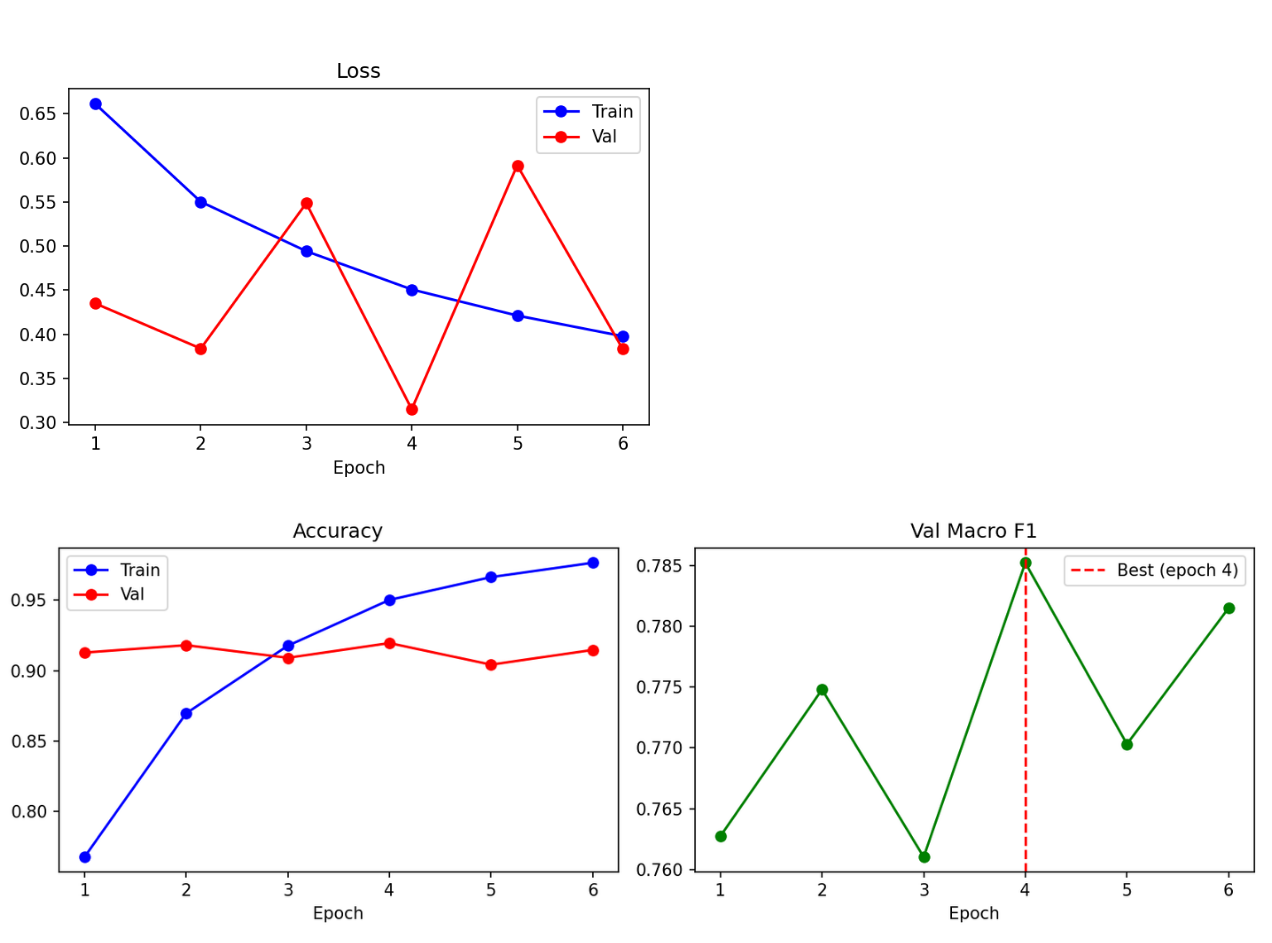
\includegraphics[width=\columnwidth]{image/figure3.png}
  \caption{Đường cong training/validation của ViAmpleHate trên ViHSD (best epoch 4, macro-F1 trên validation $=0,7852$). \texttt{training\_curves\_viamplehate.png}.}
  \label{fig:curves}
\end{figure}

\subsection{Phân tích định tính}
Để minh họa cụ thể các kiểu lỗi, Bảng~\ref{tab:qual} liệt kê một số dạng bình luận tiêu biểu. Đây là các ví dụ dựng lại theo những phạm trù quan sát được; trong phiên bản camera-ready, nên thay bằng mẫu test thực đã ẩn danh. Xu hướng chung là ViAmpleHate hỗ trợ tốt nhất khi một target tường minh đi kèm một attack predicate, và kém nhất với những trường hợp thù ghét hàm ẩn, tức không nêu target nào và cũng không có từ attack lộ liễu.

\begin{table}[tbp]
  \centering
  \small
  \begin{tabular}{p{0.34\linewidth}ccc}
    \toprule
    \textbf{Kiểu bình luận} & \textbf{Tgt} & \textbf{Atk} & \textbf{Gold} \\
    \midrule
    Nhãn nhóm + vị từ thù địch       & yes & yes & HATE \\
    Lời tục, không target nhóm       & no  & yes & NON \\
    Mỉa mai/hàm ẩn, không cue lộ     & no  & no  & HATE \\
    Nhãn nhóm trong context trung tính & yes & no & NON \\
    \bottomrule
  \end{tabular}
  \caption{Các trường hợp minh họa (ví dụ dựng lại; nên thay bằng ví dụ thực). Tgt/Atk = có hiện diện target/attack cue.}
  \label{tab:qual}
\end{table}

% HÌNH 5 — Ma trận nhầm lẫn ViHSD: baseline so với đề xuất.
\begin{figure*}[tp]
  \centering
  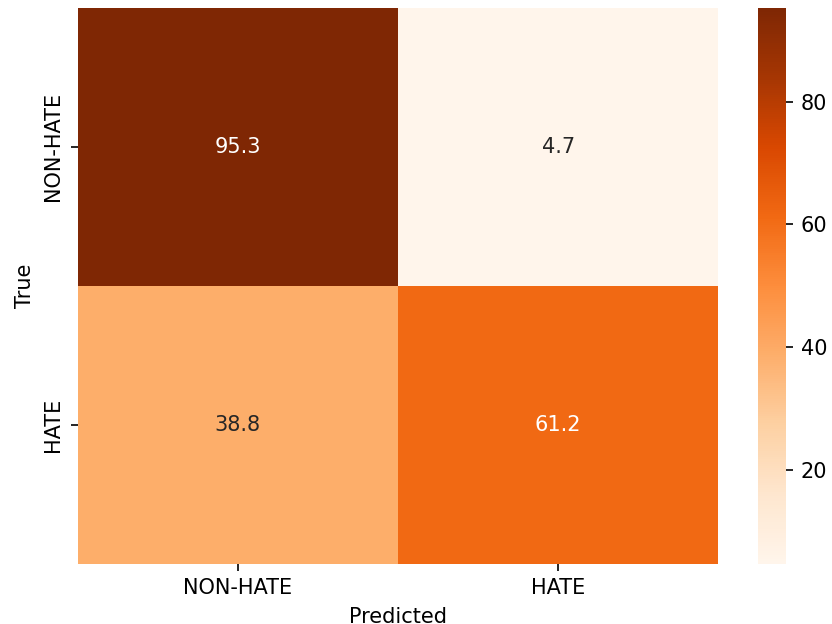
\includegraphics[width=0.45\linewidth]{image/figure4a.png}\hfill
  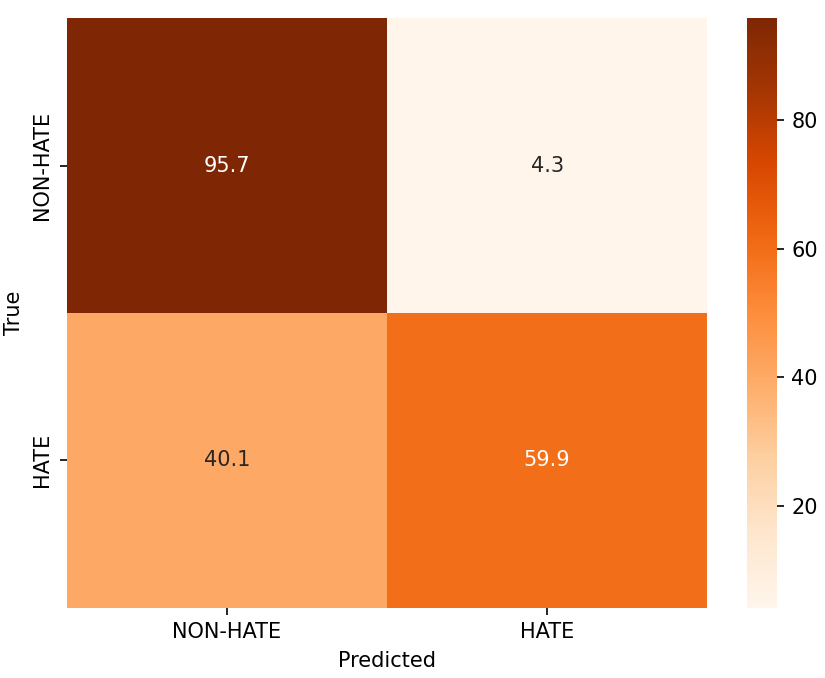
\includegraphics[width=0.45\linewidth]{image/figure4b.png}
  \caption{Confusion matrix trên ViHSD: AmpleHate baseline (trái) so với ViAmpleHate (phải). \texttt{confusion\_matrix\_amplehate.png} và \texttt{confusion\_matrix\_viamplehate.png}; lưu ý số false positive của lớp HATE giảm.}
  \label{fig:cm}
\end{figure*}

\begin{table}[tbp]
  \centering
  \small
  \setlength{\tabcolsep}{4pt}
  \begin{tabular}{llrrr}
    \toprule
    \textbf{Dữ liệu} & \textbf{Lớp} & \textbf{P} & \textbf{R} & \textbf{F1} \\
    \midrule
    ViHSD & NON-HATE & 0.9541 & 0.9574 & 0.9558 \\
    ViHSD & HATE     & 0.6177 & 0.5988 & 0.6081 \\
    VOZ   & NON-HATE & 0.9638 & 0.9719 & 0.9678 \\
    VOZ   & HATE     & 0.7347 & 0.6803 & 0.7065 \\
    \bottomrule
  \end{tabular}
  \caption{Kết quả theo từng lớp của ViAmpleHate (tập test, một lần chạy).}
  \label{tab:perclass}
\end{table}

\subsection{Thảo luận}
Có ba điểm đáng chú ý. Thứ nhất, trên ViHSD, thay đổi chủ yếu là tái cân bằng precision/recall hơn là một mức tăng đồng đều: precision của HATE tăng ($0{,}5972\!\to\!0{,}6177$) trong khi recall \emph{giảm} ($0{,}6119\!\to\!0{,}5988$). Precision cao hơn có lợi khi cáo buộc nhầm là tốn kém, nhưng recall thấp hơn đồng nghĩa với bỏ sót nhiều hơn; lựa chọn điểm cân bằng phù hợp phụ thuộc vào bối cảnh triển khai. Nhóm chỉ báo cáo ở một threshold đơn và để dành phân tích precision--recall đầy đủ cho sau. Trên VOZ-HSD, nơi độ phủ cao hơn, recall của HATE cũng cao hơn (0,6803; Bảng~\ref{tab:perclass}). Thứ hai, mức tăng lớn hơn trên VOZ-HSD đi kèm accuracy giảm cho thấy mô hình đánh đổi accuracy của lớp đa số để cải thiện chất lượng ở lớp thiểu số, một đánh đổi thường phù hợp khi lớp thiểu số là trọng tâm. Thứ ba, quan hệ giữa độ phủ cue và mức cải thiện gợi mở một hướng nâng cấp ít tốn kém, đó là mở rộng và tinh chỉnh cue bank, dù vẫn cần kiểm chứng thêm (Mục~\ref{sec:coverage}).

\subsection{Phân tích lỗi}
Nhóm chia các lỗi còn lại thành bảy nhóm thường gặp. \textbf{(1) Xúc phạm nhưng không phải thù ghét:} lời lăng mạ hoặc lời tục nhắm vào một cá nhân, không phải một nhóm được bảo vệ; khi mô hình đặt trọng số quá lớn vào attack cue, false positive dễ xuất hiện. \textbf{(2) Thù ghét hàm ẩn:} bình luận không có slur, thực thể có tên hay attack predicate lộ liễu, nhưng vẫn thể hiện thù địch qua mỉa mai, định kiến hoặc ngữ cảnh xã hội chung; lúc này việc trích cue gần như không tìm được tín hiệu để attend. \textbf{(3) Tham chiếu target mơ hồ:} đại từ và danh từ chỉ nhóm cũng xuất hiện trong bình luận trung tính hoặc hài hước, nên một target cue thiếu ngữ cảnh thù địch dễ khiến mô hình dự đoán nhầm thành HATE. \textbf{(4) Cue chưa phủ đủ:} tiếng lóng thay đổi nhanh, biến thể chính tả, viết tắt, lời tục sáng tạo hoặc bị kiểm duyệt là những hiện tượng mà cue bank cố định khó bao quát hết, dẫn tới false negative. \textbf{(5) Lệch token và span:} span của NER, kết quả tách từ và subword tokenization của PhoBERT có thể không trùng khớp, nhất là với các cụm nhiều từ, khiến cue đôi khi khớp sai vị trí. \textbf{(6) Nhạy cảm với threshold:} threshold tinh chỉnh trên validation có thể không còn phù hợp khi phân phối dữ liệu thay đổi. \textbf{(7) Mất cân bằng lớp:} khi số mẫu dương quá ít, lỗi ở lớp thiểu số vẫn dai dẳng dù đã dùng weighted loss và tinh chỉnh threshold. Các hướng khắc phục gồm mở rộng cue bank bằng khai thác dữ liệu có kiểm chứng thủ công, ghi log dự đoán theo từng mẫu (gate, độ phủ cue, confidence) để phân tích false positive/negative, bổ sung span supervision hoặc phát hiện mỉa mai, và áp dụng probability calibration.

\section{Kết luận và hướng phát triển}
ViAmpleHate thích ứng AmpleHate cho tiếng Việt thông qua trích xuất target tiếng Việt, tách riêng hai kênh target/attack cue, relation-bank attention và relation injection thích ứng (kèm một chỉnh sửa batched-attention ở mức triển khai), đồng thời huấn luyện bằng weighted cross-entropy kết hợp contrastive loss. Trên ViHSD và VOZ-HSD, mô hình cải thiện cả macro-F1 lẫn HATE-F1 so với baseline AmpleHate và các baseline TF-IDF, BiLSTM, PhoBERT-CNN, rõ nhất ở lớp thiểu số của VOZ-HSD; mức tăng trên ViHSD còn nhỏ và cần xác nhận lại bằng so sánh đa seed. Phân tích cho thấy các mức cải thiện gắn với độ phủ target, vốn được cue bank tiếng Việt nâng lên khoảng hai bậc độ lớn so với NER tiếng Anh; tuy nhiên, đây mới là liên hệ tương quan và chưa thể khẳng định nhân quả. Bài học rộng hơn là target-aware chỉ phát huy đầy đủ khi được thích ứng với hình thái bề mặt của ngôn ngữ đích. Hướng phát triển tiếp theo gồm tự động khai thác cue bank kèm kiểm chứng thủ công, phân tích lỗi ở mức từng mẫu, bổ sung span supervision và phát hiện mỉa mai, mở rộng sang thiết lập multi-label/multi-target theo tinh thần ViTHSD, và áp dụng probability calibration để ổn định hơn khi chuyển miền.

% \section*{Lời cảm ơn}

\bibliography{custom}

\appendix

\section{Hyperparameters}
\label{sec:hparams}
\begin{table}[H]
  \centering
  \small
  \setlength{\tabcolsep}{3pt}
  \begin{tabular}{@{}>{\raggedright\arraybackslash}p{0.50\columnwidth}>{\raggedright\arraybackslash}p{0.47\columnwidth}@{}}
    \toprule
    \textbf{Tham số} & \textbf{Giá trị} \\
    \midrule
    Encoder & \texttt{vinai/phobert-base} (768-d) \\
    NER tiếng Việt & \texttt{NlpHUST/\allowbreak ner-vietnamese-\allowbreak electra-base} \\
    max\_len & 256 \\
    LR (encoder / head) & 2e-5 / 5e-5 \\
    Dropout & 0.1 \\
    Effective batch & 32 (16 $\times$ grad-accum 2) \\
    Epoch & tối đa 8 (chọn tốt nhất theo macro-F1 trên val) \\
    $\alpha$ (contrastive) & 0.1 \\
    Class weight $w_c$ & inverse freq.\ $N/(C\,n_c)$ \\
    Contrastive margin $m$ & 0.5 \\
    Label smoothing & 0.05 \\
    Seed / số lần chạy & 42 / một lần chạy \\
    ViHSD best epoch / val F1 / thr. & 4 / 0.7852 / 0.43 \\
    \bottomrule
  \end{tabular}
  \caption{Toàn bộ siêu tham số.}
  \label{tab:hparams}
\end{table}

\section{Ví dụ cue bank}
\label{sec:cuebank}
Hai bank đầy đủ---16 target cue và 24 attack cue---được phát hành kèm mã nguồn và liệt kê trong báo cáo đi kèm; tại đây, nhóm chỉ nêu một vài ví dụ an toàn ASCII. \textbf{Target cue} mang tính tham chiếu và bản thân không hàm ý thù ghét: các cách gọi người/nhóm phi chính thức, nhãn vùng miền và nhân khẩu, đại từ nhóm. \textbf{Attack cue} là các vị từ thù địch thể hiện sự khinh miệt, phi nhân tính hóa hoặc ăn bám (ví dụ \texttt{khinh}, \texttt{an\_bam}). Hai loại cue này được lưu trong các bank tách biệt (Mục~\ref{sec:cue}).

\section{Khả năng tái lập}
\label{sec:repro}
Mọi mô hình dựa trên PhoBERT đều dùng chung \texttt{vinai/phobert-base}; điểm khác nhau giữa baseline và ViAmpleHate nằm ở cách mô hình hóa target/relation, phép tính attention, fusion và loss. Checkpoint tốt nhất được chọn theo macro-F1 trên validation, còn threshold cho lớp HATE được chọn trên validation rồi cố định cho test. Việc khớp cue chỉ chạy một lần ở bước tiền xử lý, theo kiểu khớp trọn chuỗi token với dòng token của PhoBERT.

\end{document}
